\section{Load balancing}
\label{sec:heuristics}

% introduction

For parallel computations on distributed memory systems, the global domain is partitioned into several subdomains, each of which is assigned to a single process. Such a mesh decomposition is showcased in Fig.~\ref{fig:decomposition}.

\begin{figure}
\centering
\begin{subfigure}[t]{.49\textwidth}
  \centering
  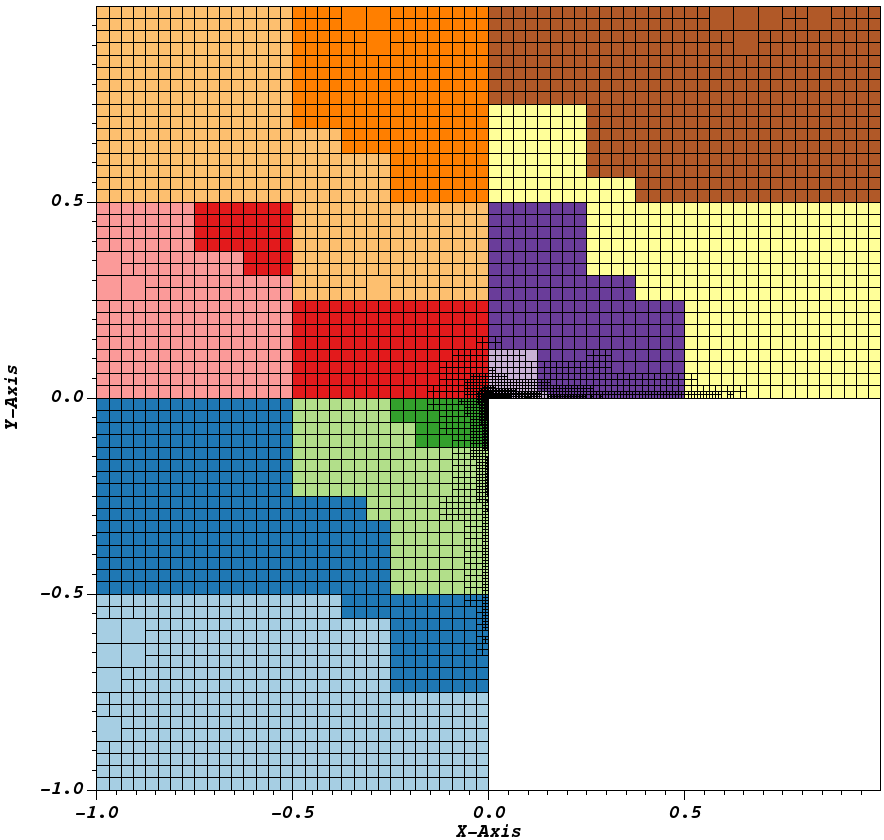
\includegraphics[width=\textwidth]{figures/results/corner-2d-error-hp-legendre-05_subdomain12.png}
  \caption{Constant weighting.}
\end{subfigure}
\begin{subfigure}[t]{.49\textwidth}
  \centering
  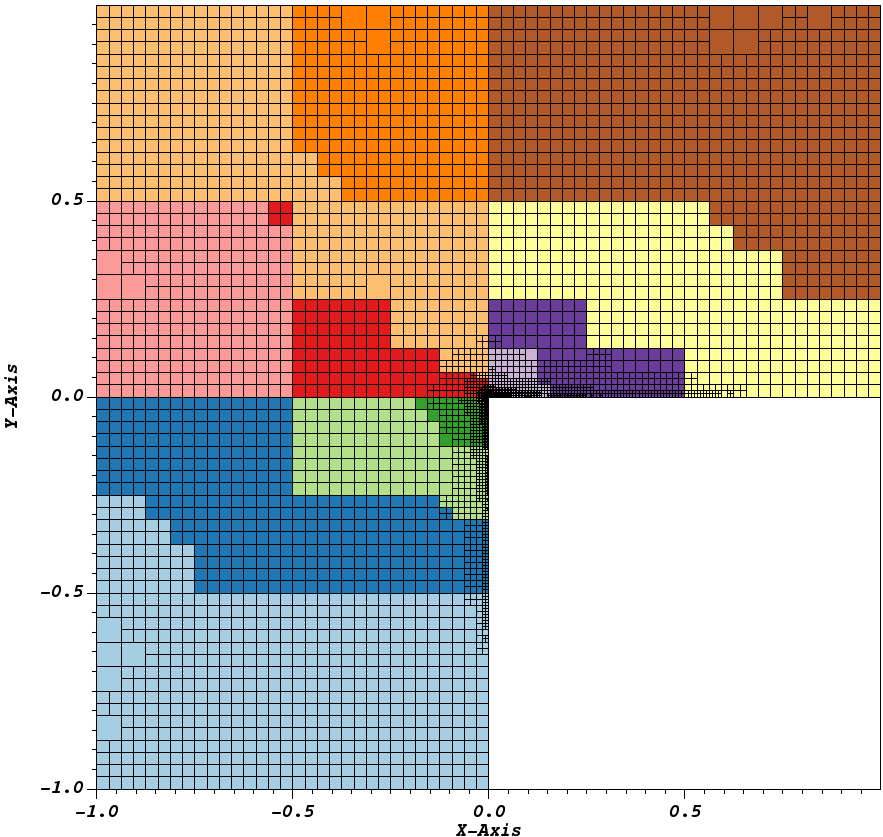
\includegraphics[width=\textwidth]{figures/results/corner-2d-error-hp-legendre-05_subdomain12_customweighting.png}
  \caption{Weighting with an individually potentiated number of \glspl{dof}, i.e., $\propto n_\text{dofs}^{1.9}$.}
\end{subfigure}
\caption{Decomposition of the mesh after six iterations with the Legendre coefficient decay strategy on 12 \gls{mpi} processes with various cell weighting. Each color represents a different subdomain.}
\label{fig:decomposition}
\end{figure}

Proper load balancing is necessary for an efficient use of all computational resources. Especially on \gls{hpc} systems with lots of available processors, this is a critical feature. For \hp-adaptive \gls{fem}, we presented approaches for load balancing in Sec.~\ref{sec:balancing} by assigning weights to each individual cell and balancing the accumulated weight among all processes. We relate the weight to the number of \glspl{dof} on each cell potentiated by an exponent that we will determine in the upcoming investigations. In other words, cell weights are chosen proportional to $n_\text{dofs}^c$ with the exponent $c$ to be ascertained.

Although all three \hp-adaptive strategies have demonstrated a similar performance as shown in Sec.~\ref{sec:errorvsperformance}, we pick only one adaptation strategy for our parallel investigations. We choose the smoothness estimation strategy based on the decay of Legendre coefficients as the most efficient one for this purpose.

% system specifications

Investigations are carried out on the JURECA supercomputer \parencite{krause2016,jureca}. Each computing node is equipped with two Intel\textsuperscript{\textregistered} Xeon\textsuperscript{\textregistered} E5-2680 v3 processors with twelve cores running at 2.5GHz and either 128GB, 256GB or 512GB of memory. With simultaneous multithreading, a total of 48 threads are available per node. Communication between nodes happens via a Mellanox EDR InfiniBand high-speed network. More information on the configuration of the supercomputer can be found here \textcite{jureca}.

In this section, our investigations are performed on two distinct nodes, which provide a total of 96 threads and involve communication between two physically independent memory segments. We expect that this setup yields representative results that can be extrapolated on even larger problem sizes.

Further, we use a 'flat' \gls{mpi} model: Every thread will be assigned to an individual \gls{mpi} process and no additional thread parallelization is invoked. Although \dealii{} provides such a feature via Intel\textsuperscript{\textregistered} \gls{tbb}, we refrain from using it to measure the pure \gls{mpi} performance for all parallel analyses in this work.

% problem specifications

To qualify our problem for parallel computations, we need to increase its size drastically. The problem is initialized with nine global refinements and gets adapted in twelve iterations. For the strategy with the Legendre coefficient decay, this results in a total number of 46,369,440 \glspl{dof}, so that in the best case each process will be assigned to a number of 483,015 \glspl{dof} on average. Each type of finite element from the provided collection is represented at least once in the mesh.

This advanced scenario will form the basis of our investigations to see how different weighting exponents affect the wall time, and which one provides a minimum. With serialization, we ensure that each of these runs conforms to the same conditions. Again, to mitigate the impact of temporary slowdowns on the supercomputer due to high loads on memory and network bandwidth, we repeat each run for a total of five times and take the minimum wall time in each category over all runs.

% results

For varying weighting exponents, we compare the wall times of the full adaptation cycle and its relevant sections
%For resumed scenarios in which the mesh will be partitioned according to weights with different weighting exponents, we compare the wall time of critical sections of the program as well as the total wall time
%between runs with different weighting exponents
in Fig.~\ref{fig:weights}.

\begin{figure}
\centering
\begin{tikzpicture}
\begin{axis}[
  xlabel=Weighting exponent,
  ylabel=Wall time {[seconds]},
  legend pos=outer north east]

\addplot table [y=full cycle, x=weighting exponent, col sep=comma] {data/weight/weight.csv};
\addlegendentry{full cycle};

\addplot table [y=assembly, x=weighting exponent, col sep=comma] {data/weight/weight.csv};
\addlegendentry{assemble linear system};

\addplot table [y=solve, x=weighting exponent, col sep=comma] {data/weight/weight.csv};
\addlegendentry{linear solver and preconditioner};
\end{axis}
\end{tikzpicture}
\caption[Wall times for load balancing with varying weighting exponents.]{Wall times of a complete adaptation cycle and those parts relevant for load balancing. The problem has a number of about 46 million \glspl{dof} and is solved on 2 nodes or 96 \gls{mpi} processes. Weights proportional to $n_\text{dofs}^c$ will be assigned to each cell with varying exponents $c$.}
\label{fig:weights}
\end{figure}

As discussed in Sec.~\ref{sec:balancing}, the assembly of the equation system and the its solution are identified as the critical sections whose wall time is affected by the number of \glspl{dof}. We see that the solution of the equation system takes about 90\% of the total wall time and is the crucial factor for proper load balancing. The minimal wall time for both solver and the full cycle is reached with a weighting exponent of $c = 1.9$.

We were dissatisfied to find the minimum wall time of the solver at such a high exponent, since we expected $c = 1$ for an efficient solver.
%This may be related to the implementation of the preconditioner combined with the disorder that \hp-adaptive methods cause in the system matrix.
On closer reflection, this is not surprising considering the large number of non-zero entries in the system matrix caused by high order finite elements, which the current implementation of the preconditioner does not handle efficiently.
Further, we were expecting a minimum in the assembly at about $c = 2$, but found it was decaying at even higher exponents. We have no explanation for this behavior. Analyzing the effect of cell weighting on each individual section of the program
%the load balancing
will be subject of further investigations.

% Next step
%We set an weighting expoenent to a value of $c = 1.9$ for the following considerations regarding scalability.
